\documentclass[conference]{IEEEtran}

\usepackage[T1]{fontenc}
\usepackage[utf8]{inputenc}
\usepackage{amsmath,amssymb}
\usepackage{graphicx}
\usepackage{booktabs}
\usepackage{tabularx}
\usepackage{multirow}
\usepackage{siunitx}
\usepackage{cite}
\usepackage{xurl}
\usepackage{tikz}
\usetikzlibrary{arrows.meta,positioning,fit,calc}

\graphicspath{{../reduced/TFG/}}
\sisetup{detect-all=true}

\title{Prior-Anchored Deep Learning for Dense UAV Air-to-Ground Channel Knowledge Maps}

\author{\IEEEauthorblockN{Guillem Moreno Garcia, Evgenii Vinogradov, Sergi Abadal}}

\begin{document}
\maketitle

\begin{abstract}
Channel knowledge maps (CKMs) promise fast environment-aware radio planning, but
dense air-to-ground CKM generation remains difficult when path loss, delay
spread, and angular spread must all be predicted over unseen urban layouts. This
paper condenses a full thesis project into its final technical line: a strict
city-holdout evaluation protocol, train-only calibrated physical/statistical
priors, and a bounded residual neural model with a Gaussian-mixture residual
head. The final model predicts \(513\times513\) dense maps from topology,
geometric masks, UAV height, and frozen priors. On held-out cities it reaches
\SI{1.6519}{dB} path-loss RMSE, \SI{26.5570}{ns} delay-spread RMSE, and
\(11.3854^\circ\) angular-spread RMSE, improving the frozen priors for all
targets. The result supports a hybrid design principle: use calibrated priors
for stable radial and visibility-dependent structure, and reserve neural
capacity for bounded local residuals and target-distribution mismatch.
\end{abstract}

\begin{IEEEkeywords}
channel knowledge maps, UAV communications, radio-map prediction, path loss,
delay spread, angular spread, Gaussian mixture models, physics-informed
learning.
\end{IEEEkeywords}

\section{Introduction}

Channel knowledge maps (CKMs) store or predict radio-channel quantities as
functions of position and environment, enabling faster planning and adaptation
than repeated ray tracing or exhaustive measurements \cite{zengx2021ckm,
ckmtutorial2024}. In UAV-enabled 6G networks, CKMs are especially attractive
because altitude changes both the geometry and the line-of-sight probability of
the link \cite{khawaja_survey,saboor2025height}. A practical CKM surrogate,
however, must generalize to urban layouts not seen during training and must not
hide hard propagation regimes behind a single global score.

The thesis behind this paper began as a generic dense image-to-image learning
problem, but that formulation was not sufficient. Early U-Net and cGAN models
could draw plausible maps, yet their physical errors remained large under a
ground-only metric. PMNet/PMHHNet-style backbones improved smooth LoS structure
but did not solve NLoS mode collapse or the spike-plus-tail nature of spread
targets. The final design therefore moved away from ``bigger backbone first''
and toward a hybrid sequence:
\begin{enumerate}
\item define the evaluation contract before comparing models;
\item diagnose target distributions before choosing losses and heads;
\item calibrate strong train-only priors for predictable structure;
\item train a bounded residual model around those frozen priors.
\end{enumerate}

The contribution is not a new propagation law or a claim of universal benchmark
dominance. It is a defensible dense CKM recipe for one fixed UAV simulation
contract: strict city holdout, valid-receiver masking, explicit LoS/NLoS and
height reporting, and a final prior-anchored neural correction.

\section{Related Work}

Dense radio-map prediction has often been treated as image-to-image regression.
RadioUNet \cite{radiounet2020} established convolutional radio-map estimation
as a strong baseline; PMNet and the ICASSP path-loss challenge family further
showed that U-Net-like architectures can perform well for path-loss maps
\cite{pmnet2023,icassp2023challenge}. More recent models introduce attention,
equivariance, or domain-shift machinery, including RMTransformer
\cite{rmtransformer2025}, RadioGUNet \cite{radiogunet2025}, PathFinder
\cite{pathfinder2025}, and digital-twin radio-map generators such as AIRMap
\cite{airmap2025}. These papers provide the closest dense path-loss map
context, but they generally do not match the present contract: continuous UAV
height, strict city holdout on CKM samples, and three dense targets (path loss,
delay spread, angular spread).

CKM work itself emphasizes that a radio map is not merely an image but a
position-indexed channel side-information object \cite{zengx2021ckm,
ckmtutorial2024,ckmdata2024}. This is why the evaluation protocol matters as
much as the neural architecture. A random image split can reward memorization of
urban morphology, whereas a city split tests whether the learned propagation
surrogate transfers to unseen layouts.

Physics-informed and hybrid methods address a different weakness of pure image
regression: the model should not need to rediscover stable propagation effects
from pixels alone. ReVeal \cite{reveal2025} uses physics-informed constraints
for radio-environment mapping, while classical air-to-ground, COST/Hata, and
two-ray models encode known distance, height, reflection, and elevation-angle
structure \cite{rappaport,goldsmith,cost231,alhourani2014,khawaja_survey,
tr38901,wocc2021}. This paper uses those models only as shape priors; all
deployment coefficients are calibrated from training cities under the same CKM
masking convention used at inference.

The final neural head is also informed by distribution-aware wireless learning.
Heteroscedastic regression \cite{kendall2017uncertainties}, mixture-density
wireless predictors \cite{saleh2021probabilistic,garciamarti2020mixture,
lee2024timevarying}, and recent stochastic radio-map models
\cite{radiodiff2025} all point to the same issue: NLoS and spread targets are
not well represented by a single symmetric residual. For spread targets, the
closest external references are often scalar channel-parameter predictors or
standard channel-model statistics \cite{tr38901,winner2,cai2019,
izydorczyk2019}, not dense maps, so they are not used as direct CKM
benchmarks here.

\section{Task and Evaluation Protocol}

Each sample is a \(513\times513\) urban topology map from the ray-traced CKM
setting used throughout the thesis. The carrier is fixed at
\SI{7.125}{GHz}, so frequency is not a learned variable; the main transmitter
degree of freedom is height. There is one UAV transmitter at the map centre.
The transmitter horizontal position is fixed, but its antenna height
\(h_{\mathrm{tx}}\) varies by sample and is treated as a central conditioning
variable rather than as metadata. The spatial resolution is
\SI{1}{m}\(\times\)\SI{1}{m} per pixel. Every non-building pixel is treated as
an active receiver location, with the receiver antenna placed at
\(h_{\mathrm{rx}}=\SI{1.5}{m}\) above the ground. Building pixels are excluded
from the receiver set rather than treated as easy zero-error targets. The model
predicts three aligned dense maps:
\[
  y_t \in \{\mathrm{PL~(dB)}, \mathrm{DS~(ns)}, \mathrm{AS~(deg)}\}.
\]
Let \(m_i(p)=1\) if pixel \(p\) of sample \(i\) is one of these valid ground
receivers, and zero otherwise. For a split \(\mathcal{S}\), the
target-specific pixel-weighted RMSE is
\begin{equation}
  \mathrm{RMSE}_t =
  \sqrt{
  \frac{\sum_{i\in\mathcal{S}}\sum_p m_i(p)
  \left(\hat{y}_{i,t}(p)-y_{i,t}(p)\right)^2}
  {\sum_{i\in\mathcal{S}}\sum_p m_i(p)}}.
  \label{eq:rmse}
\end{equation}

The split is city-based rather than random over pixels or tiles. This matters:
random splits would allow the model to see nearly identical urban morphology
during training and testing. The final held-out test split contains 2590
samples from cities not used to optimize model weights. Validation is used for
model selection; test is used only for the final generalization claim.

\subsection{Quantized Targets and Continuous Outputs}

The released CKM targets are not ideal real-valued measurements. Path loss is
stored on an approximately \SI{1}{dB} grid, while delay spread and angular
spread are strongly integer-valued and visibly staircase-like in many maps. The
model outputs are not quantized to these grids: the residual network emits
continuous values, and all reported metrics compare those continuous outputs
against the stored targets. This matters for interpretation. The final
path-loss MAE is \SI{0.9298}{dB}, close to the \SI{1}{dB} label step, while
the path-loss RMSE is \SI{1.6519}{dB} because RMSE emphasizes the remaining
hard tails. A cleaner or less quantized dataset would likely expose more of
the continuous surrogate's resolution, especially for small residual
improvements and spread-map boundaries.

\section{Method}

\subsection{Why the Final Method Is Hybrid}

The development path exposed three distinct target regimes. First, LoS path
loss contains stable radial, height-dependent, and coherent two-ray structure.
Second, NLoS path loss is not just a smooth residual; it is a blocked-link
distribution-placement problem. Third, delay spread and angular spread contain
near-zero LoS spikes and NLoS-heavy tails. Thus a single point-regression CNN is
asked to solve three different statistical problems at once.

The final method uses a division of labour. Frozen priors provide a strong mean
prediction for structure that can be calibrated reliably from training data.
The neural model receives those priors and learns bounded residual corrections.
This makes the prior useful but not magical: distribution-first neural models
showed that NLoS structure can be learned without explicit priors when the
target distribution is represented correctly. The priors are reintroduced
because they are cheaper, more stable, and more auditable for the predictable
part of the map.

\begin{figure*}[t]
\centering
\resizebox{0.96\textwidth}{!}{%
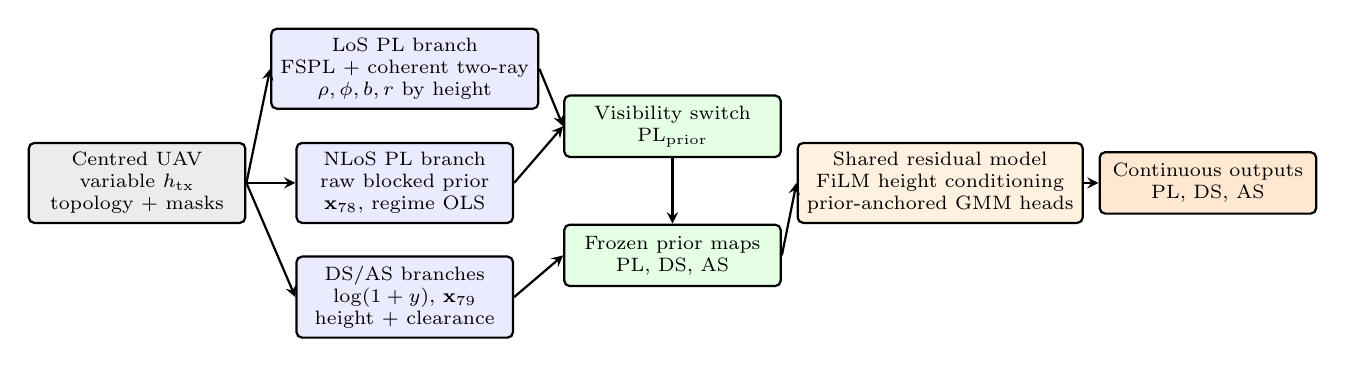
\begin{tikzpicture}[
  >=stealth,
  font=\scriptsize,
  box/.style={draw, thick, rounded corners=2pt, rectangle, minimum width=2.75cm, minimum height=0.78cm, align=center},
  input/.style={box, fill=gray!15},
  prior/.style={box, fill=blue!8},
  cal/.style={box, fill=green!10},
  model/.style={box, fill=orange!12},
  arr/.style={->, thick}
]
\node[input] (support) at (0,0) {Centred UAV\\variable \(h_{\mathrm{tx}}\)\\topology + masks};
\node[prior] (los) at (3.4,1.45) {LoS PL branch\\FSPL + coherent two-ray\\\(\rho,\phi,b,r\) by height};
\node[prior] (nlos) at (3.4,0) {NLoS PL branch\\raw blocked prior\\\(\mathbf{x}_{78}\), regime OLS};
\node[prior] (spread) at (3.4,-1.45) {DS/AS branches\\\(\log(1+y)\), \(\mathbf{x}_{79}\)\\height + clearance};
\node[cal] (switch) at (6.8,0.72) {Visibility switch\\\(\mathrm{PL}_{\mathrm{prior}}\)};
\node[cal] (stack) at (6.8,-0.92) {Frozen prior maps\\PL, DS, AS};
\node[model] (net) at (10.2,0) {Shared residual model\\FiLM height conditioning\\prior-anchored GMM heads};
\node[input, fill=orange!18] (out) at (13.6,0) {Continuous outputs\\PL, DS, AS};

\draw[arr] (support.east) -- (los.west);
\draw[arr] (support.east) -- (nlos.west);
\draw[arr] (support.east) -- (spread.west);
\draw[arr] (los.east) -- (switch.west);
\draw[arr] (nlos.east) -- (switch.west);
\draw[arr] (switch.south) -- (stack.north);
\draw[arr] (spread.east) -- (stack.west);
\draw[arr] (stack.east) -- (net.west);
\draw[arr] (net.east) -- (out.west);
\end{tikzpicture}}
\caption{Compact thesis-style pipeline. The transmitter is always centred, but
its height varies by sample. Frozen height-aware priors are produced first and
then used as channels for the final prior-anchored residual GMM model.}
\label{fig:pipeline}
\end{figure*}

\subsection{Frozen Priors}

The path-loss prior combines a coherent two-ray LoS branch with a calibrated
NLoS branch. The LoS side follows the textbook direct-plus-ground-reflected
field structure \cite{rappaport,goldsmith}; the NLoS side uses empirical
urban and A2G attenuation shapes as a starting point \cite{cost231,
alhourani2014,khawaja_survey,tr38901}. The UAV remains horizontally centred,
so \(d_{2D}\) is the per-pixel distance from the centre transmitter to each
receiver. The height \(h_{\mathrm{tx}}\), however, changes from sample to
sample and is one of the main physical degrees of freedom in the method. For
receiver height \(h_{\mathrm{rx}}\) and carrier frequency \(f_{\mathrm{MHz}}\),
the direct and reflected distances are
\begin{equation}
\begin{aligned}
d_{\mathrm{LoS}}
&=\sqrt{d_{2D}^2+(h_{\mathrm{tx}}-h_{\mathrm{rx}})^2},\\
d_{\mathrm{ref}}
&=\sqrt{d_{2D}^2+(h_{\mathrm{tx}}+h_{\mathrm{rx}})^2}.
\end{aligned}
\label{eq:path-distances}
\end{equation}
The LoS branch starts from
\begin{equation}
\mathrm{FSPL}
=32.45+20\log_{10}\!\left(\frac{d_{\mathrm{LoS}}}{1000}\right)
+20\log_{10}(f_{\mathrm{MHz}})
\label{eq:fspl-paper}
\end{equation}
and adds an effective coherent reflection correction
\begin{equation}
C_{\mathrm{2ray}}
=-20\log_{10}\!\left|
1+\rho(h_{\mathrm{tx}})\frac{d_{\mathrm{LoS}}}{d_{\mathrm{ref}}}
e^{-j(k(d_{\mathrm{ref}}-d_{\mathrm{LoS}})+\phi(h_{\mathrm{tx}}))}
\right|.
\label{eq:tworay-paper}
\end{equation}
The final LoS prior is
\begin{equation}
\mathrm{PL}_{\mathrm{LoS}}
=\mathrm{FSPL}+C_{\mathrm{2ray}}+b(h_{\mathrm{tx}})
+r(d_{2D},h_{\mathrm{tx}}),
\label{eq:los-prior-paper}
\end{equation}
where \(b\) is a height-dependent bias and \(r\) is a smoothed radial residual
fit. This LoS prior is not FSPL alone and it is not a learned linear
regressor. The direct distance \(d_{\mathrm{LoS}}\) sets the free-space
baseline, the image-source distance \(d_{\mathrm{ref}}\) supplies the
ground-reflected path, and \(k(d_{\mathrm{ref}}-d_{\mathrm{LoS}})\) is the
extra phase accumulated by that reflected wave. The train-calibrated functions
\(\rho(h_{\mathrm{tx}})\) and \(\phi(h_{\mathrm{tx}})\) are effective
reflection amplitude and phase curves, fitted in \SI{5}{m} UAV-height bins,
smoothed across bins, and linearly interpolated to the actual sample height at
inference. The terms \(b(h_{\mathrm{tx}})\) and
\(r(d_{2D},h_{\mathrm{tx}})\) are outside the textbook two-ray expression:
they remove, respectively, a remaining height-dependent offset and a smooth
range-dependent residual; these terms are also stored as height-conditioned
calibration curves rather than as one global correction.

The LoS calibration is deliberately structured rather than fully flexible. It
is fitted only on valid LoS ground pixels from training cities. First, the
effective reflection amplitude \(\rho\) and phase \(\phi\) are fitted in
\SI{5}{m} UAV-height bins to reproduce the ring-like constructive and
destructive interference visible in LoS path-loss maps. Second, the per-height
bias \(b\) removes a remaining vertical offset after the coherent two-ray fit.
Third, the radial residual table \(r(d_{2D},h_{\mathrm{tx}})\) averages the
remaining error by distance from the centred transmitter, smooths it across
radius, clips it to a small dB range, and stores it by height. At inference,
the actual \(h_{\mathrm{tx}}\) selects/interpolates these calibration curves,
so the LoS prior changes continuously with antenna height even though the UAV
horizontal coordinate remains fixed at the map centre.

The NLoS prior starts from the maximum of COST231-like and A2G-NLoS raw
terms. The COST/Hata-shaped term is used as an urban-macro shape prior,
\begin{equation}
\begin{aligned}
\mathrm{PL}_{C}
={}&46.3+33.9\log_{10}(f_{\mathrm{MHz}})
\\
&-13.82\log_{10}(h_{\mathrm{tx}})
-a(h_{\mathrm{rx}})\\
&+\eta(h_{\mathrm{tx}})\log_{10}(d_{\mathrm{km}})+3,\\
\eta(h_{\mathrm{tx}})
={}&44.9-6.55\log_{10}(h_{\mathrm{tx}}),
\end{aligned}
\label{eq:cost-paper}
\end{equation}
where \(C\) denotes the COST231-shaped branch,
\(d_{\mathrm{km}}=\max(d_{2D}/1000,0.001)\), and \(a(h_{\mathrm{rx}})\)
is the usual mobile-height correction. The A2G envelope is
\begin{equation}
\begin{aligned}
\mathrm{PL}_{\mathrm{A2G,NLoS}}
={}&\lambda_0(h_{\mathrm{tx}},f)+\beta_{\mathrm{NLoS}}\\
&+A_{\mathrm{NLoS}}
\exp\!\left(-\frac{90-\theta^\circ}{\tau_{\mathrm{NLoS}}}\right),
\end{aligned}
\label{eq:a2g-paper}
\end{equation}
with \(\lambda_0=20\log_{10}(4\pi h_{\mathrm{tx}}f/c)\). The raw blocked-link
prior is the conservative envelope
\begin{equation}
P_0
=
\mathrm{PL}_{\mathrm{NLoS,raw}}
=
\max(\mathrm{PL}_{C},\mathrm{PL}_{\mathrm{A2G,NLoS}}).
\label{eq:nlos-raw-paper}
\end{equation}
This maximum is deliberately pessimistic: if the urban empirical curve predicts
stronger attenuation it is kept, and if the elevation-aware A2G envelope is
larger it is kept instead. The raw prior is then corrected by train-only
regime-wise linear calibration:
\begin{equation}
\mathrm{PL}_{\mathrm{NLoS}}
=\operatorname{clip}(\mathbf{x}_{78}^{\top}\mathbf{w}_{78,r},20,180).
\label{eq:nlos-prior-paper}
\end{equation}
The path-loss prior is therefore not one formula with a small correction. It
is two different calibrated feature extractors. The LoS side calibrates
height-binned two-ray amplitude/phase, height bias, and radial residual curves.
The NLoS side uses the raw blocked-link prior only as one feature in a
15-term morphology vector:
\begin{equation}
\begin{aligned}
\mathbf{x}_{78}=[&
P_0^2,P_0,\log(1+d_{2D}),\rho_{15},\rho_{41},h_{15},h_{41},\\
&\rho_{41}h_{41},\rho_{41}\log(1+d_{2D}),n_{15},n_{41},
s,\theta,n_{41}\theta,1]^{\top},
\end{aligned}
\label{eq:x78-paper}
\end{equation}
where \(P_0\) is the raw NLoS prior, \(\rho_{15}\) and \(\rho_{41}\) are the
fractions of building pixels in \(15\times15\) and \(41\times41\) windows,
\(h_{15}\) and \(h_{41}\) are local building-height summaries, \(n_{15}\) and
\(n_{41}\) summarize local NLoS support, \(s\) is a shadow/blocker proxy, and
\(\theta\) is the normalized elevation-angle feature. The interaction
\(\rho_{41}h_{41}\) lets dense tall neighborhoods differ from sparse tall
ones, \(\rho_{41}\log(1+d_{2D})\) lets density matter differently with range,
and \(n_{41}\theta\) activates when obstruction and elevation jointly matter.
The constant \(1\) is the regime-wise bias term. The
deployed path-loss prior is selected by the geometric visibility mask:
\begin{equation}
\mathrm{PL}_{\mathrm{prior}}
=m_{\mathrm{LoS}}\mathrm{PL}_{\mathrm{LoS}}
+(1-m_{\mathrm{LoS}})\mathrm{PL}_{\mathrm{NLoS}}.
\label{eq:path-prior-paper}
\end{equation}
The regime index \(r\) is not a learned latent class. It is selected from
observable scene descriptors: topology/morphology class, LoS/NLoS state, and
antenna-height group, with fallback calibrations when an exact regime has too
few training pixels. Thus the prior is auditable: one can inspect the raw
blocked estimate \(P_0\), the local morphology terms, the selected regime, and
the final linear correction separately.

\begin{table*}[!t]
\centering
\caption{Term-by-term interpretation of the main frozen-prior quantities.}
\label{tab:prior-term-meanings}
\scriptsize
\begin{tabularx}{\textwidth}{p{0.16\textwidth}p{0.22\textwidth}X}
\toprule
Term & Prior block & Interpretation \\
\midrule
\(d_{\mathrm{LoS}}\) & LoS PL & 3D direct transmitter--receiver distance; sets the FSPL baseline. \\
\(d_{\mathrm{ref}}\) & LoS PL & Image-source reflected distance; gives the length and attenuation of the single ground-reflected ray. \\
\(C_{\mathrm{2ray}}\) & LoS PL & Coherent direct-plus-reflected correction; negative values mean constructive gain over FSPL and positive values mean fading loss. \\
\(\rho(h_{\mathrm{tx}}),\phi(h_{\mathrm{tx}})\) & LoS PL & Height-interpolated effective reflection amplitude and phase, calibrated from CKM rather than assumed from a fixed material. \\
\(b(h_{\mathrm{tx}})\) & LoS PL & Height-dependent dB offset remaining after the coherent two-ray fit. \\
\(r(d_{2D},h_{\mathrm{tx}})\) & LoS PL & Smoothed radial residual profile; removes systematic range-dependent error left by the two-ray model. \\
\(P_0\) & NLoS PL & Raw blocked-link path-loss prior before morphology calibration. \\
\(\rho_k,h_k,n_k\) & NLoS PL and spreads & Local building density, local building height, and local NLoS support in a \(k\times k\) window. \\
\(b_{41},c_{41},t_{41}\) & Spreads & Blocker depth, transmitter clearance, and fraction of buildings taller than the link-line proxy. \\
\(\theta_{\mathrm{norm}},\theta_{\mathrm{inv}}\) & Spreads & Elevation angle and its low-elevation complement; low elevation is where street-canyon and rooftop interactions are stronger. \\
\bottomrule
\end{tabularx}
\end{table*}

The delay-spread and angular-spread priors are fitted in a transformed domain,
\begin{equation}
z=\log(1+y),
\qquad
\hat y=\exp(\hat z)-1,
\label{eq:spread-transform-paper}
\end{equation}
because both standard channel models and the CKM histograms make spread
quantities more regular in log space \cite{tr38901,winner2}. The released
spread maps have a near-zero mass plus a long tail: LoS direct-path pixels
cluster near zero, while blocked or rooftop-scattered pixels create rare but
important large values. Their raw prior is
\begin{equation}
\begin{aligned}
z^{(0)}
={}&\log(1+b^{\mathrm{nat}}_q)
+b_{\mathrm{top}}
+a_1\log(1+d_{2D})+a_2\theta_{\mathrm{inv}} \\
&+a_3\rho_{41}+a_4h_{41}+a_5n_{41}
+a_6n_{41}\theta_{\mathrm{inv}},
\end{aligned}
\label{eq:spread-raw-paper}
\end{equation}
where \(q\) is the LoS/NLoS state. The native anchor
\(b^{\mathrm{nat}}_q\) gives a different starting scale to LoS and NLoS
pixels, \(b_{\mathrm{top}}\) shifts the baseline by topology class,
\(\log(1+d_{2D})\) captures range growth, \(\theta_{\mathrm{inv}}\) increases
the prior for low-elevation links, and \(\rho_{41}\), \(h_{41}\), and
\(n_{41}\) summarize local building density, height, and NLoS support. This
raw log prior is intentionally simple; it encodes the expected spike-plus-tail
shape before CKM-specific calibration. A 23-term feature vector then augments
\(z^{(0)}\) with range, elevation, height, multi-scale morphology,
blocker-depth, clearance, and interaction terms:
\begin{equation}
\begin{aligned}
\mathbf{x}_{79}=[&
(z^{(0)})^2,z^{(0)},\log(1+d_{2D}),\theta_{\mathrm{norm}},
\theta_{\mathrm{inv}},h,h^2,\\
&\rho_{15},\rho_{41},h_{15},h_{41},n_{15},n_{41},
n_{41}\log(1+d_{2D}),\\
&\rho_{41}\theta_{\mathrm{inv}},b_{41},1,c_{41},t_{41},
\theta_{\mathrm{norm}}\rho_{41},\\
&c_{41}\theta_{\mathrm{inv}},t_{41}\rho_{41},t_{41}n_{41}]^{\top}.
\end{aligned}
\label{eq:x79-paper}
\end{equation}
Here \(h\) is normalized UAV height, \(b_{41}\) is a local blocker-depth
summary, \(c_{41}\) is transmitter clearance over nearby buildings, and
\(t_{41}\) is the fraction of locally taller buildings. These height terms are
not incidental: they tell the spread prior whether the centred UAV is above the
local skyline, near rooftop level, or below nearby high-rise clutter. The
quadratic raw prior terms let the calibration bend the initial log-domain
estimate, while the interaction terms represent cases where range, low
elevation, dense buildings, and NLoS support become harmful together. The
calibrated log prior is ridge-regularized per metric and regime:
\begin{equation}
\hat{\mathbf{w}}_{79,r}
=
\left(\mathbf{X}^{\top}\mathbf{X}
+\lambda\mathbf{D}^{\top}\mathbf{D}\right)^{-1}
\mathbf{X}^{\top}\mathbf{z}.
\label{eq:ridge-paper}
\end{equation}
The calibrated log prior is then
\(\hat z=\mathbf{x}_{79}^{\top}\hat{\mathbf{w}}_{79,r}\).
The diagonal regularizer \(\mathbf{D}\) keeps the calibrated curve close to the
raw prior unless the training residuals consistently justify a correction. In
practice this matters for the spread targets: a flexible unregularized fit can
chase rare high-spread pixels, whereas the ridge fit keeps the near-zero LoS
bulk and the NLoS tail connected to the same physical features.
All calibrations use training cities only. The spread-prior dictionary contains 114
fitted regime keys, but this number is not one Cartesian product. Per spread
metric, the exact grid contributes \(6\) topology classes \(\times\) \(2\)
visibility states \(\times\) \(3\) height bins \(=36\) exact keys. The
implementation then adds \(12\) height-collapsed topology/visibility fallbacks,
\(6\) topology-wide fallbacks, \(2\) global visibility fallbacks, and \(1\)
fully global fallback, for \(57\) keys per metric and \(114\) keys across DS
and AS. Height is handled differently across the frozen estimators: the LoS PL
branch interpolates its fitted \SI{5}{m} height-bin curves, while the NLoS PL
and spread branches use discrete antenna-height regimes with fallback keys;
the spread model also keeps continuous height, clearance, and taller-building
features inside \(\mathbf{x}_{79}\). This heavy calibration is the point: the prior stores many small
decisions about morphology, visibility, and height before the neural residual
is trained. The same-protocol frozen-prior results are \SI{1.7516}{dB} LoS PL,
\SI{3.3967}{dB} NLoS PL, \SI{1.9246}{dB} overall PL, \SI{28.10}{ns} DS, and
\(13.74^\circ\) AS. The final neural model receives only the resulting prior
maps as channels; the handcrafted features remain inside the frozen prior
estimators rather than becoming additional learned inputs.

\subsection{Prior-Anchored Residual Model}

The neural model receives nine aligned channels: topology, LoS mask, NLoS
mask, ground mask, combined path-loss prior, LoS path-loss prior, NLoS
path-loss prior, delay-spread prior, and angular-spread prior. Height is
encoded with sinusoidal features and injected through FiLM modulation
\cite{perez2018film}, so the final network can adapt the residual correction
continuously between the calibrated height regimes instead of learning one
height-agnostic correction. The backbone is a shared U-Net-style
encoder-decoder with GroupNorm, FiLM conditioning, and task-specific residual
heads.

The height path mirrors the detailed thesis implementation. The scalar
\(h_{\mathrm{tx}}\) is expanded to a 32-dimensional sinusoidal code using
16 log-spaced frequencies over the UAV-height range,
\begin{equation}
\mathbf{e}(h_{\mathrm{tx}})
=
\left[
\sin\!\frac{h_{\mathrm{tx}}}{f_i},
\cos\!\frac{h_{\mathrm{tx}}}{f_i}
\right]_{i=1}^{16}
\in\mathbb{R}^{32},
\label{eq:height-embed-paper}
\end{equation}
then mapped by an MLP to a \(\mathbb{R}^{160}\) condition vector. Each FiLM
site projects this vector to channel-wise scale and shift parameters and
modulates a feature map as
\begin{equation}
\mathbf{X}'=\mathbf{X}\odot(1+\mathbf{g})+\mathbf{b}.
\label{eq:film-paper}
\end{equation}
Encoder FiLM uses the height condition directly; decoder FiLM and the global
task heads use a fused condition formed from the height code and the pooled
bottleneck context. Thus the same centred topology can receive different
residual corrections when the UAV is at \SI{30}{m}, \SI{150}{m}, or
\SI{350}{m}.

\begin{figure*}[!t]
\centering
\resizebox{0.98\textwidth}{!}{%
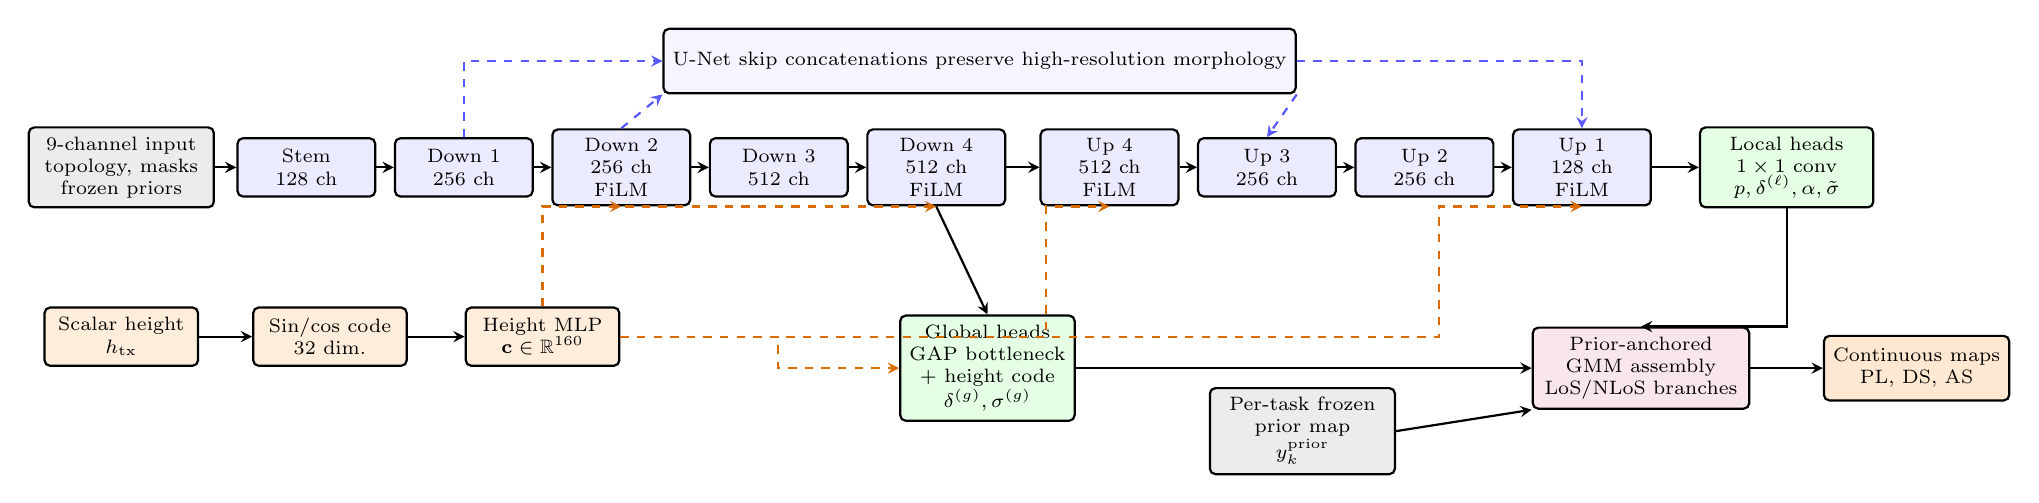
\begin{tikzpicture}[
  >=stealth,
  font=\scriptsize,
  block/.style={draw, thick, rounded corners=2pt, rectangle, minimum width=1.75cm, minimum height=0.74cm, align=center, fill=blue!8},
  cond/.style={draw, thick, rounded corners=2pt, rectangle, minimum width=1.95cm, minimum height=0.74cm, align=center, fill=orange!14},
  head/.style={draw, thick, rounded corners=2pt, rectangle, minimum width=2.2cm, minimum height=0.82cm, align=center, fill=green!10},
  gmm/.style={draw, thick, rounded corners=2pt, rectangle, minimum width=2.75cm, minimum height=1.0cm, align=center, fill=purple!10},
  prior/.style={draw, thick, rounded corners=2pt, rectangle, minimum width=2.35cm, minimum height=0.82cm, align=center, fill=gray!15},
  arr/.style={->, thick},
  condarr/.style={->, thick, dashed, orange!85!black},
  skiparr/.style={->, thick, dashed, blue!65}
]
\node[prior] (input) at (0,0.8) {9-channel input\\topology, masks\\frozen priors};
\node[block] (stem) at (2.35,0.8) {Stem\\128 ch};
\node[block] (down1) at (4.35,0.8) {Down 1\\256 ch};
\node[block] (down2) at (6.35,0.8) {Down 2\\256 ch\\FiLM};
\node[block] (down3) at (8.35,0.8) {Down 3\\512 ch};
\node[block] (bott) at (10.35,0.8) {Down 4\\512 ch\\FiLM};
\node[block] (up4) at (12.55,0.8) {Up 4\\512 ch\\FiLM};
\node[block] (up3) at (14.55,0.8) {Up 3\\256 ch};
\node[block] (up2) at (16.55,0.8) {Up 2\\256 ch};
\node[block] (up1) at (18.55,0.8) {Up 1\\128 ch\\FiLM};
\node[head] (local) at (21.15,0.8) {Local heads\\\(1\times1\) conv\\\(p,\delta^{(\ell)},\alpha,\tilde\sigma\)};

\draw[arr] (input) -- (stem);
\draw[arr] (stem) -- (down1);
\draw[arr] (down1) -- (down2);
\draw[arr] (down2) -- (down3);
\draw[arr] (down3) -- (bott);
\draw[arr] (bott) -- (up4);
\draw[arr] (up4) -- (up3);
\draw[arr] (up3) -- (up2);
\draw[arr] (up2) -- (up1);
\draw[arr] (up1) -- (local);

\node[cond] (height) at (0,-1.35) {Scalar height\\\(h_{\mathrm{tx}}\)};
\node[cond] (embed) at (2.65,-1.35) {Sin/cos code\\32 dim.};
\node[cond] (hmlp) at (5.35,-1.35) {Height MLP\\\(\mathbf{c}\in\mathbb{R}^{160}\)};
\node[head] (global) at (11.0,-1.75) {Global heads\\GAP bottleneck\\+\ height code\\\(\delta^{(g)},\sigma^{(g)}\)};
\node[prior] (taskprior) at (15.0,-2.55) {Per-task frozen\\prior map\\\(y_k^{\mathrm{prior}}\)};
\node[gmm] (assembly) at (19.3,-1.75) {Prior-anchored\\GMM assembly\\LoS/NLoS branches};
\node[prior, fill=orange!18] (out) at (22.8,-1.75) {Continuous maps\\PL, DS, AS};

\draw[arr] (height) -- (embed);
\draw[arr] (embed) -- (hmlp);
\draw[condarr] (hmlp.north) |- (down2.south);
\draw[condarr] (hmlp.north) |- (bott.south);
\draw[condarr] (hmlp.east) -- ++(2.0,0) |- (global.west);
\draw[condarr] (hmlp.east) -- ++(5.4,0) |- (up4.south);
\draw[condarr] (hmlp.east) -- ++(10.4,0) |- (up1.south);

\draw[arr] (bott.south) -- (global.north);
\draw[arr] (global.east) -- (assembly.west);
\draw[arr] (local.south) |- (assembly.north);
\draw[arr] (taskprior.east) -- (assembly.south west);
\draw[arr] (assembly.east) -- (out.west);

\node[prior, fill=blue!4, minimum width=5.2cm] (skip) at (10.9,2.15)
{U-Net skip concatenations preserve high-resolution morphology};
\draw[skiparr] (down1.north) |- (skip.west);
\draw[skiparr] (down2.north) -- (skip.south west);
\draw[skiparr] (skip.south east) -- (up3.north);
\draw[skiparr] (skip.east) -| (up1.north);
\end{tikzpicture}}
\caption{Final shared deep-learning architecture adapted from the thesis
diagram. The map stack carries topology, masks, and frozen priors; the scalar
UAV height is encoded separately and injected through FiLM. A shared U-Net
produces local residual fields, pooled bottleneck features produce global GMM
parameters, and the prior-anchored GMM assembly emits continuous PL/DS/AS maps.}
\label{fig:dl-architecture}
\end{figure*}

The head keeps the two-stage logic of the distribution-first predecessors, but
moves it into residual space around the frozen prior. The global stage asks:
``what residual distribution does this whole map, height, and topology imply?''
The local stage asks: ``where should each residual component be placed in the
\(513\times513\) map?'' This is the key distinction from a direct U-Net
regressor. The network does not directly overwrite the prior with a free-form
map; it predicts a small residual distribution and then assigns that residual
pixel by pixel.

For each task \(k\), visibility region \(r\in\{\mathrm{LoS},\mathrm{NLoS}\}\),
component \(j\in\{1,2,3\}\), and pixel \(p\), the global head receives the
pooled bottleneck and fused height/context vector and outputs
\[
  \{\pi^{(g)}_{k,r,j},\delta^{(g)}_{k,r,j},\sigma^{(g)}_{k,r,j}\}_{j=1}^{3}.
\]
After the implementation transforms, \(\pi^{(g)}\) is a map-level residual
mixture distribution, \(\delta^{(g)}\) is a bounded global residual offset, and
\(\sigma^{(g)}\) is a bounded global uncertainty scale. The local head receives
the full-resolution decoder feature map and outputs
\[
  \{p_{k,r,j}(p)\}_{j=1}^{3},\quad
  \delta^{(\ell)}_{k,r}(p),\quad
  \alpha_{k,r}(p),\quad
  \tilde\sigma_{k,r}(p).
\]
Here \(p_{k,r,j}(p)\) is the per-pixel component assignment, the local residual
\(\delta^{(\ell)}\) shifts all components at that pixel, \(\alpha\) is an
anchor gate initialized with bias \(-2\) so the model starts close to the
prior, and \(\tilde\sigma\) is the local uncertainty term. This extends the
distribution-aware line of work from scalar mixture predictors to dense
residual maps \cite{saleh2021probabilistic,garciamarti2020mixture,
lee2024timevarying}. The native residual is clipped by target and visibility:
\begin{equation}
\Delta_{k,r,j}(p)
=\operatorname{clip}\!\left(
\delta^{(g)}_{k,r,j}+\delta^{(\ell)}_{k,r}(p),
-\delta_{\max,k,r},\delta_{\max,k,r}
\right),
\label{eq:delta-paper}
\end{equation}
with caps of \(7/25\) dB for PL LoS/NLoS, \(20/20\) ns for DS, and
\(17^\circ/15^\circ\) for AS. The component mean is anchored to the frozen
prior:
\begin{equation}
\begin{aligned}
\mu^{\mathrm{native}}_{k,r,j}(p)
&=y^{\mathrm{prior}}_k(p)
+\alpha_{k,r}(p)\Delta_{k,r,j}(p),\\
0&\leq \alpha_{k,r}(p)\leq 1.
\end{aligned}
\label{eq:mu-paper}
\end{equation}
PL is modeled in native dB space, while DS and AS use the log transform in
Eq.~\eqref{eq:spread-transform-paper}. The deterministic map used for RMSE is
the mixture expectation:
\begin{equation}
\hat z_{k,r}(p)
=\sum_{j=1}^3p_{k,r,j}(p)\mu_{k,r,j}(p).
\label{eq:gmm-expectation-paper}
\end{equation}
For PL, \(\hat y_{k,r}=\hat z_{k,r}\). For DS and AS, the output is mapped
back with \(\hat y_{k,r}=\exp(\hat z_{k,r})-1\).
The final map selects the LoS or NLoS branch with the explicit geometric mask.
The mixture variances combine map-level and local uncertainty,
\begin{equation}
\sigma_{k,r,j}(p)
=
\sqrt{
\left(\sigma^{(g)}_{k,r,j}\right)^2
+
\left(\tilde\sigma_{k,r}(p)\right)^2
},
\label{eq:sigma-paper}
\end{equation}
with both terms constrained to \([0.05,3.0]\). During the residual/GMM stage
these variances and mixture weights define a pixel-wise likelihood; during the
final fine-tuning stage the same head remains in place but the reported output
is the deterministic expectation above.

The two mixture-weight objects have different jobs. The global weights
\(\pi^{(g)}_{k,r,j}\) describe the sample-level residual histogram and are
used by the distributional regularizer. The local weights \(p_{k,r,j}(p)\)
are the pixel-wise assignment probabilities used in the final dense map. During
the residual/GMM stage the per-pixel density is
\begin{equation}
q_{k,r}(z_k(p)\mid p)
=
\sum_{j=1}^{3}
p_{k,r,j}(p)\,
\mathcal{N}\!\left(
z_k(p);\mu_{k,r,j}(p),\sigma^2_{k,r,j}(p)
\right),
\label{eq:gmm-density-paper}
\end{equation}
and the regional NLL is the masked average of
\(-\log q_{k,r}(z_k(p)\mid p)\) over valid LoS or NLoS pixels. Separately,
the KL term bins the true residuals
\(\epsilon_k(p)=y_k(p)-y^{\mathrm{prior}}_k(p)\) into a soft empirical
histogram and compares it with the histogram implied by
\(\{\pi^{(g)}_{k,r,j},\delta^{(g)}_{k,r,j}\}\). This is what makes the head
``distribution-first'': before the decoder places values pixel by pixel, the
global branch is pressured to put mixture mass where the map residuals actually
live.

\begin{figure*}[!t]
\centering
\resizebox{0.96\textwidth}{!}{%
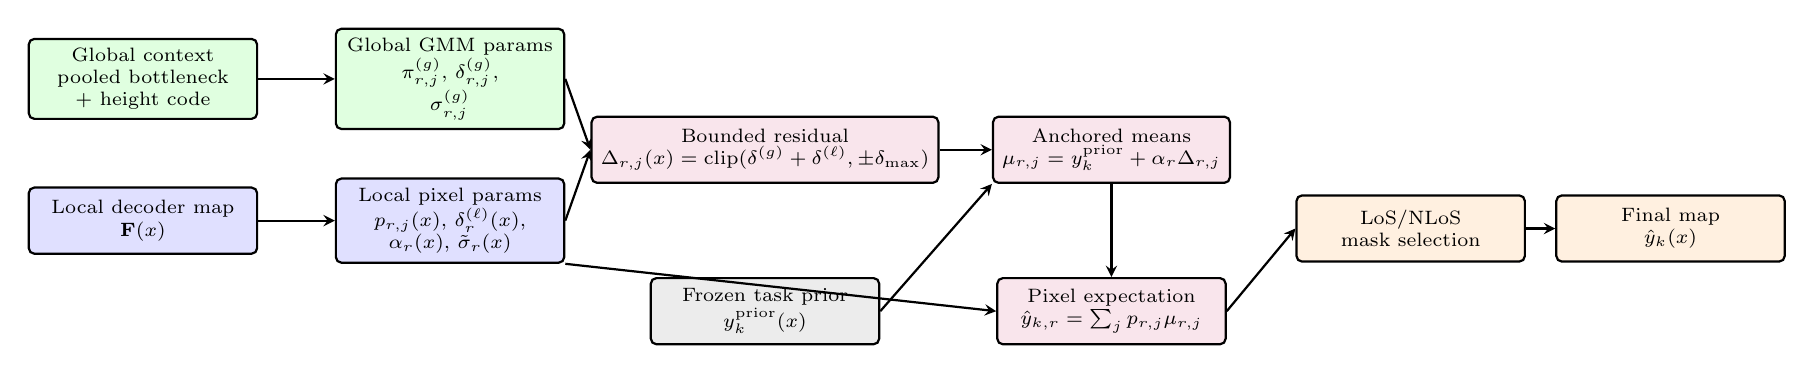
\begin{tikzpicture}[
  >=stealth,
  font=\scriptsize,
  box/.style={draw, thick, rounded corners=2pt, rectangle, minimum width=2.9cm, minimum height=0.84cm, align=center},
  global/.style={box, fill=green!12},
  local/.style={box, fill=blue!12},
  prior/.style={box, fill=gray!15},
  mix/.style={box, fill=purple!10},
  outbox/.style={box, fill=orange!12},
  arr/.style={->, thick}
]
\node[global] (g0) at (0,1.6) {Global context\\pooled bottleneck\\+\ height code};
\node[global] (g1) at (3.9,1.6) {Global GMM params\\\(\pi^{(g)}_{r,j}\), \(\delta^{(g)}_{r,j}\),\\\(\sigma^{(g)}_{r,j}\)};
\node[local] (l0) at (0,-0.2) {Local decoder map\\\(\mathbf{F}(x)\)};
\node[local] (l1) at (3.9,-0.2) {Local pixel params\\\(p_{r,j}(x)\), \(\delta^{(\ell)}_r(x)\),\\\(\alpha_r(x)\), \(\tilde\sigma_r(x)\)};
\node[mix] (resid) at (7.9,0.7) {Bounded residual\\\(\Delta_{r,j}(x)=\mathrm{clip}(\delta^{(g)}+\delta^{(\ell)},\pm\delta_{\max})\)};
\node[prior] (p0) at (7.9,-1.35) {Frozen task prior\\\(y^{\mathrm{prior}}_k(x)\)};
\node[mix] (mu) at (12.3,0.7) {Anchored means\\\(\mu_{r,j}=y^{\mathrm{prior}}_k+\alpha_r\Delta_{r,j}\)};
\node[mix] (expv) at (12.3,-1.35) {Pixel expectation\\\(\hat y_{k,r}=\sum_j p_{r,j}\mu_{r,j}\)};
\node[outbox] (sel) at (16.1,-0.3) {LoS/NLoS\\mask selection};
\node[outbox] (out) at (19.4,-0.3) {Final map\\\(\hat y_k(x)\)};

\draw[arr] (g0) -- (g1);
\draw[arr] (l0) -- (l1);
\draw[arr] (g1.east) -- (resid.west);
\draw[arr] (l1.east) -- (resid.west);
\draw[arr] (resid) -- (mu);
\draw[arr] (p0.east) -- (mu.south west);
\draw[arr] (mu.south) -- (expv.north);
\draw[arr] (l1.south east) -- (expv.west);
\draw[arr] (expv.east) -- (sel.west);
\draw[arr] (sel.east) -- (out.west);
\end{tikzpicture}}
\caption{Final prior-anchored GMM head. The global branch predicts the
sample-level residual mixture; the local branch places that distribution
pixel by pixel through component weights, residual refinements, gates and local
uncertainty. Component means are anchored to the frozen prior and the
deterministic map is the pixel-wise mixture expectation after LoS/NLoS
selection.}
\label{fig:gmm-head}
\end{figure*}

The final prior-anchored model should not be read as only the final fine-tuning loss. It has two active
training phases: a large-capacity residual/GMM stage with probabilistic losses
enabled, followed by an RMSE/MAE-dominant fine-tuning stage. The composite
objective implemented by the model is
\begin{equation}
\begin{aligned}
\mathcal{L}
={}&
\sum_k w_k\bigl(
\lambda_{\mathrm{NLL}}\mathcal{L}_{\mathrm{NLL},k}
+\lambda_{\mathrm{KL}}\mathcal{L}_{\mathrm{KL},k}
+\lambda_{\mathrm{mom}}\mathcal{L}_{\mathrm{mom},k}\\
&+\lambda_{\mathrm{anchor}}\mathcal{L}_{\mathrm{anchor},k}
+\lambda_{\mathrm{guard}}\mathcal{L}_{\mathrm{guard},k}
+\lambda_{\mathrm{out}}\mathcal{L}_{\mathrm{out},k}\\
&+\lambda_{\mathrm{RMSE}}\mathcal{L}_{\mathrm{RMSE},k}
+\lambda_{\mathrm{MAE}}\mathcal{L}_{\mathrm{MAE},k}
\bigr).
\end{aligned}
\label{eq:loss}
\end{equation}

The probabilistic terms matter during the residual/GMM stage. The NLL term
teaches the head to place mixture mass around the transformed target, the KL
and moment terms keep the mixture distribution from becoming a numerically
convenient but physically uninformative density, and the outlier-budget term
discourages a solution that spends most of its capacity on the easy bulk while
leaving large tails unconstrained. The final fine-tuning stage then disables
those terms and optimizes the deterministic mixture expectation for RMSE/MAE,
with a small anchor and guard that keep the correction close to the prior.
Table~\ref{tab:loss-roles} summarizes the roles. The selected checkpoint is
therefore reported as a deterministic RMSE improvement over the frozen priors,
not as a calibrated probabilistic predictor.

\begin{table*}[!t]
\centering
\caption{Loss terms available in the final prior-anchored objective and their practical
purpose.}
\label{tab:loss-roles}
\scriptsize
\begin{tabularx}{\textwidth}{p{0.15\textwidth}p{0.18\textwidth}X}
\toprule
Term & Active stage & Role \\
\midrule
GMM NLL & residual/GMM stage &
Fits the per-pixel mixture density in native PL space and log-transformed
spread space. \\
Distribution KL & residual/GMM stage &
Regularizes the learned mixture so it remains close to the intended
distributional structure instead of using degenerate weights or variances. \\
Moment matching & residual/GMM stage &
Encourages the expectation and spread of the mixture to agree with target
moments, stabilizing deterministic extraction from the GMM. \\
Outlier budget & residual/GMM stage &
Keeps rare large residuals visible in the objective instead of letting the
global average hide them. \\
Anchor & both stages &
Penalizes unnecessary deviation from the frozen prior; this is especially
important because the prior is already a strong calibrated predictor. \\
Prior guard & both stages &
Adds a penalty when the model becomes worse than the prior at valid pixels,
discouraging destructive corrections. \\
RMSE / MAE & both stages, dominant in final fine-tuning &
Optimizes the deterministic map reported in the final evaluation; RMSE handles
tails and MAE tracks typical absolute error. \\
\bottomrule
\end{tabularx}
\end{table*}

\begin{table}[t]
\centering
\caption{Training configuration of the final line.}
\label{tab:training}
\scriptsize
\begin{tabularx}{\linewidth}{lX}
\toprule
Item & Value \\
\midrule
Image size & \(513\times513\) \\
Input channels & 9 map channels plus height FiLM conditioning \\
Backbone & GroupNorm U-Net, base width 128, FiLM dim. 160 \\
Residual head & 3 mixture components, bounded residuals \\
Optimizer & AdamW, learning rate \(5\times10^{-5}\), weight decay 0.01 \\
Batching & batch size 1, gradient accumulation 8 \\
Loss schedule & Large-capacity residual/GMM stage plus final residual
fine-tuning; see Table~\ref{tab:loss-schedule} \\
\bottomrule
\end{tabularx}
\end{table}

\begin{table}[t]
\centering
\caption{Final prior-anchored loss schedule. The non-fine-tuned residual/GMM stage is part
of the final pipeline, even though the reported checkpoint is selected after
the deterministic fine-tuning stage.}
\label{tab:loss-schedule}
\scriptsize
\begin{tabularx}{\linewidth}{lXX}
\toprule
Setting & Residual/GMM stage & Final fine-tuning \\
\midrule
NLL / KL / moment / outlier & 1.00 / 0.25 / 0.10 / 0.02 & 0 / 0 / 0 / 0 \\
RMSE / MAE & 1.50 / 0.10 & 1.00 / 0.05 \\
Anchor / guard & 0.05 / 0.10 & 0.01 / 0.02 \\
Task weights & PL 1.0, DS 1.0, AS 1.0 & PL 1.0, DS 0.25, AS 0.25 \\
Learning rate & \(2\times10^{-4}\) & \(5\times10^{-5}\) \\
\bottomrule
\end{tabularx}
\end{table}

\section{Experimental Results}

\subsection{Main Test Results}

Table~\ref{tab:main-results} reports the final unseen-city test metrics. The
model improves the frozen prior for all three targets. Path loss is the cleanest
success case because both RMSE and MAE improve. Delay spread improves RMSE
while MAE slightly increases; this is consistent with reducing rare high-delay
errors while introducing small local shifts. Angular spread improves RMSE
strongly and is approximately neutral in MAE.

\begin{table*}[!t]
\centering
\caption{Final model test results on unseen cities. Negative \(\Delta\) means
that the residual model improves the frozen prior.}
\label{tab:main-results}
\scriptsize
\setlength{\tabcolsep}{4pt}
\begin{tabular}{lrrrrrrl}
\toprule
Target & Model RMSE & Prior RMSE & \(\Delta\)RMSE & Model MAE & Prior MAE & \(\Delta\)MAE & Unit \\
\midrule
Path loss & 1.6519 & 1.9383 & -0.2865 & 0.9298 & 1.2319 & -0.3020 & dB \\
Delay spread & 26.5570 & 28.1023 & -1.5453 & 7.9897 & 7.3033 & +0.6864 & ns \\
Angular spread & 11.3854 & 13.7416 & -2.3562 & 5.0088 & 4.9890 & +0.0198 & deg \\
\bottomrule
\end{tabular}
\end{table*}

The original numerical targets were \SI{5}{dB}, \SI{50}{ns}, and
\(20^\circ\). The final model clears all three on unseen cities. More
importantly, it does so jointly: the same network predicts PL/DS/AS instead of
using separate specialist models.

\subsection{LoS/NLoS and Split Diagnostics}

Table~\ref{tab:los-nlos} separates valid pixels by the geometric visibility
mask. The residual model improves the prior in both LoS and NLoS pixels for all
targets. This is important because global RMSE could otherwise hide a failure
in the physically hard NLoS subset.

\begin{table}[t]
\centering
\caption{Final test RMSE separated by LoS and NLoS pixels.}
\label{tab:los-nlos}
\scriptsize
\begin{tabular}{llrrr}
\toprule
Target & Scope & Model & Prior & \(\Delta\) \\
\midrule
PL & LoS & 1.4675 & 1.7519 & -0.2844 \\
PL & NLoS & 3.1482 & 3.5143 & -0.3661 \\
DS & LoS & 25.4419 & 27.4851 & -2.0432 \\
DS & NLoS & 29.2045 & 29.6157 & -0.4112 \\
AS & LoS & 12.3510 & 15.2818 & -2.9308 \\
AS & NLoS & 8.4424 & 8.6614 & -0.2191 \\
\bottomrule
\end{tabular}
\end{table}

The validation/test sanity check is also useful. Validation stores the model
selection values; the test row is the real generalization result. Delay spread
worsens more on test because the held-out city mix contains harder high-delay
cases. The frozen delay-spread prior shows the same validation-to-test
worsening, confirming that this is a city-mix effect rather than an evaluator
change.

\begin{table}[t]
\centering
\caption{Validation versus held-out test check for the same selected model.}
\label{tab:val-test}
\scriptsize
\begin{tabular}{lrrrr}
\toprule
Split & Samples & PL RMSE & DS RMSE & AS RMSE \\
\midrule
Validation & 2750 & 1.6157 & 22.1061 & 11.3782 \\
Test & 2590 & 1.6519 & 26.5570 & 11.3854 \\
\bottomrule
\end{tabular}
\end{table}

\subsection{Prior and Split Breakdowns}

The frozen priors are strong enough to deserve their own reporting. They are
not simply baselines for the final neural model; they encode most of the stable
geometry and therefore determine what residual problem the network sees.
Table~\ref{tab:pl-prior-height} shows the height dependence of the calibrated
path-loss prior. This is not post-hoc stratification: UAV height is part of the
estimator itself through the centred geometry, elevation angle, height-binned
calibration, and final FiLM conditioning. The trend is strongest in NLoS: the
low-altitude bin remains the hardest because many receivers are blocked by
local urban structure, while high UAVs see fewer deep shadow pockets.
Table~\ref{tab:spread-prior-height} shows the matching spread-prior pattern.
Delay spread in particular collapses with altitude, from \SI{39.90}{ns}
overall in the lowest bin to \SI{3.70}{ns} above \SI{300}{m}.

\begin{table}[!t]
\centering
\caption{Calibrated path-loss prior RMSE by UAV height.}
\label{tab:pl-prior-height}
\scriptsize
\begin{tabular}{lrrrr}
\toprule
Height bin & Overall & LoS & NLoS & Samples \\
\midrule
12--50 m & 2.180 & 1.797 & 3.756 & 1211 \\
50--150 m & 1.936 & 1.785 & 3.228 & 2634 \\
150--300 m & 1.680 & 1.666 & 2.259 & 786 \\
300--500 m & 1.627 & 1.619 & 2.255 & 362 \\
\bottomrule
\end{tabular}
\end{table}

\begin{table}[!t]
\centering
\caption{Calibrated spread-prior RMSE by UAV height.}
\label{tab:spread-prior-height}
\scriptsize
\begin{tabular}{llrrr}
\toprule
Height bin & Metric & Overall & LoS & NLoS \\
\midrule
12--50 m & DS & 39.90 & 43.04 & 35.13 \\
50--150 m & DS & 27.17 & 26.72 & 28.29 \\
150--300 m & DS & 8.70 & 8.79 & 8.13 \\
300--500 m & DS & 3.70 & 3.80 & 2.76 \\
\midrule
12--50 m & AS & 15.69 & 18.81 & 9.93 \\
50--150 m & AS & 14.19 & 15.89 & 8.41 \\
150--300 m & AS & 10.39 & 11.07 & 4.49 \\
300--500 m & AS & 8.85 & 9.34 & 2.85 \\
\bottomrule
\end{tabular}
\end{table}

The path-loss prior also varies by topology. Its overall RMSE ranges from
\SI{1.43}{dB} in open sparse low-rise maps to \SI{2.97}{dB} in dense block
high-rise maps. The NLoS branch is hardest in sparse vertical and dense
high-rise regimes, reaching \SI{3.91}{dB} and \SI{4.09}{dB}; the overall
pixel-weighted prior remains \SI{1.92}{dB}.

The final residual model improves the priors consistently across data splits,
not only on the validation split used for model selection. Table~\ref{tab:split-delta}
reports the model-minus-prior RMSE deltas. The test row is the main generalization claim. The
all-city row is not used for model selection, but it checks that the gain is
not a held-out split artifact.

\begin{table}[!t]
\centering
\caption{RMSE improvement over frozen priors by split. Negative values mean
the residual model improves the prior.}
\label{tab:split-delta}
\scriptsize
\setlength{\tabcolsep}{3pt}
\begin{tabular}{lrrrr}
\toprule
Split & Samples & PL & DS & AS \\
\midrule
Train & 10840 & -0.2895 & -2.0157 & -2.3578 \\
Validation & 2750 & -0.2758 & -1.3433 & -2.4396 \\
Test & 2590 & -0.2865 & -1.5453 & -2.3562 \\
All & 16180 & -0.2867 & -1.8406 & -2.3710 \\
\bottomrule
\end{tabular}
\end{table}

The all-city subexpert audit groups samples by morphology
(\texttt{open}, \texttt{mixed}, \texttt{dense}) and antenna-height bin. It is
a stricter check than the global row because it asks whether the residual model
helps across the deployed prior regimes rather than only in one easy subset.
Table~\ref{tab:subexpert-delta} reports RMSE deltas for the nine groups. All
entries are negative, so the residual correction improves every morphology and
height group for all three targets.

\begin{table}[!t]
\centering
\caption{All-city final-model RMSE deltas by morphology/height subexpert.
Negative values mean the final model improves the frozen prior.}
\label{tab:subexpert-delta}
\scriptsize
\setlength{\tabcolsep}{3pt}
\begin{tabular}{lrrrr}
\toprule
Group & Samples & PL & DS & AS \\
\midrule
\texttt{dense/high} & 1957 & -0.3602 & -0.6473 & -2.6405 \\
\texttt{dense/low} & 2018 & -0.3359 & -1.5779 & -2.3994 \\
\texttt{dense/mid} & 2055 & -0.3288 & -1.4074 & -2.8587 \\
\texttt{mixed/high} & 2156 & -0.2931 & -0.6794 & -2.3186 \\
\texttt{mixed/low} & 2060 & -0.2745 & -2.8379 & -2.5845 \\
\texttt{mixed/mid} & 2094 & -0.2781 & -2.0522 & -2.8200 \\
\texttt{open/high} & 1272 & -0.2721 & -0.5428 & -1.2874 \\
\texttt{open/low} & 1318 & -0.2363 & -3.1170 & -2.0271 \\
\texttt{open/mid} & 1250 & -0.2941 & -1.5789 & -1.7804 \\
\bottomrule
\end{tabular}
\end{table}

\subsection{Why Distribution Diagnostics Matter}

Fig.~\ref{fig:gmm-fit} shows the diagnostic that changed the modeling strategy:
LoS and NLoS path loss do not form a single easy Gaussian map target. The
distribution-first predecessor modeled the marginal with GMM heads and showed
that the NLoS collapse was not inevitable. The final model keeps this lesson
but anchors the residual around explicit priors.

The internal diagnostic numbers are kept as scale references, not as final
claims. The distribution-first path-loss GMM experts reached \SI{4.43}{dB} LoS
and \SI{3.34}{dB} NLoS pixel-aggregate RMSE, showing that NLoS collapse was a
modeling choice rather than a necessity. The distribution-first spread experts
reached \SI{30.96}{ns} delay-spread RMSE and \(11.78^\circ\) angular-spread
RMSE, motivating log-domain and mixture-aware treatment of spread targets. The
frozen priors then provided stronger anchors: \SI{1.9246}{dB} path-loss RMSE,
\SI{28.10}{ns} delay-spread RMSE, and \(13.74^\circ\) angular-spread RMSE.

\begin{figure}[t]
\centering

\includegraphics[width=\linewidth]{img/thesis_figures/results_addendum/try76_los_vs_nlos_distribution.png}
\caption{Path-loss target GMM fits by topology expert. The diagnostic exposed
different LoS/NLoS marginals and motivated distribution-aware heads before
returning to prior-anchored residual learning.}
\label{fig:gmm-fit}
\end{figure}

For spread targets, quantized labels make visual and RMSE interpretation harder.
The released delay and angular maps are integer-valued; smooth predictions can
be penalized across staircase-like target boundaries even when the morphology is
plausible. This does not invalidate RMSE, but it warns against overinterpreting
small local residuals.

\subsection{External Metric Context}

Table~\ref{tab:soa} places the final path-loss result beside the closest
available path-loss-side references. The table is deliberately compact and
cautious: datasets, height assumptions, target definitions, and splits differ.
No scalar indoor or link-level spread predictor is used as a direct dense-map
leaderboard.

\begin{table}[t]
\centering
\caption{Compact comparison with nearby path-loss-side metrics.}
\label{tab:soa}
\scriptsize
\setlength{\tabcolsep}{3pt}
\begin{tabularx}{\linewidth}{p{0.26\linewidth}p{0.25\linewidth}X}
\toprule
Reference & PL-side metric & Reading / caveat \\
\midrule
RadioUNet \cite{radiounet2020} &
\SI{1.6}{dB}--\SI{3.1}{dB} equivalent PL RMSE &
Final PL is in this band; no UAV height or spread targets. \\
RadioGUNet \cite{radiogunet2025} &
\SI{1.304}{dB} DPM; \SI{1.936}{dB} IRT &
Final PL is between those values; outdoor RadioMapSeer setting. \\
PMNet / ICASSP \cite{pmnet2023,icassp2023challenge} &
\SI{1.38}{dB} converted score &
Final PL is \(1.20\times\) worse; scale context only, no joint spread prediction. \\
ReVeal \cite{reveal2025} &
\SI{1.95}{dB} outdoor sparse-measurement RMSE &
Final PL is \(1.18\times\) better; sparse mapping rather than dense generation. \\
RMTransformer / PathFinder \cite{rmtransformer2025,pathfinder2025} &
\(\approx\SI{1.82}{dB}\) / \(\approx\SI{1.19}{dB}\) converted references &
Useful scale checks, but random/specialized splits and different assumptions. \\
AIRMap \cite{airmap2025} &
Path-gain error \(<\SI{4}{dB}\) against ray tracing &
Same broad digital-twin motivation, but path gain and \(200\times200\) maps. \\
\textbf{Final model (ours)} &
\textbf{\SI{1.6519}{dB} PL; \SI{26.5570}{ns} DS; \(11.3854^\circ\) AS} &
\textbf{Strict CKM city holdout, centred variable-height UAV, dense \(513\times513\) PL/DS/AS.} \\
\bottomrule
\end{tabularx}
\end{table}

The fair conclusion is narrow but useful. The final path-loss number is in the
same band as strong dense radio-map references, while the spread results should
be interpreted primarily against same-protocol internal baselines because no
external dense CKM PL/DS/AS benchmark was found.

\subsection{Qualitative Residual Behavior}

Fig.~\ref{fig:panel} is the qualitative check. The model receives the frozen
prior and predicts a correction. The useful visual evidence is not merely that
the prediction resembles the target; it is that the correction row tends to
anti-correlate with the prior-error row, which is the expected behavior of a
prior-anchored residual corrector.

\begin{figure*}[t]
\centering
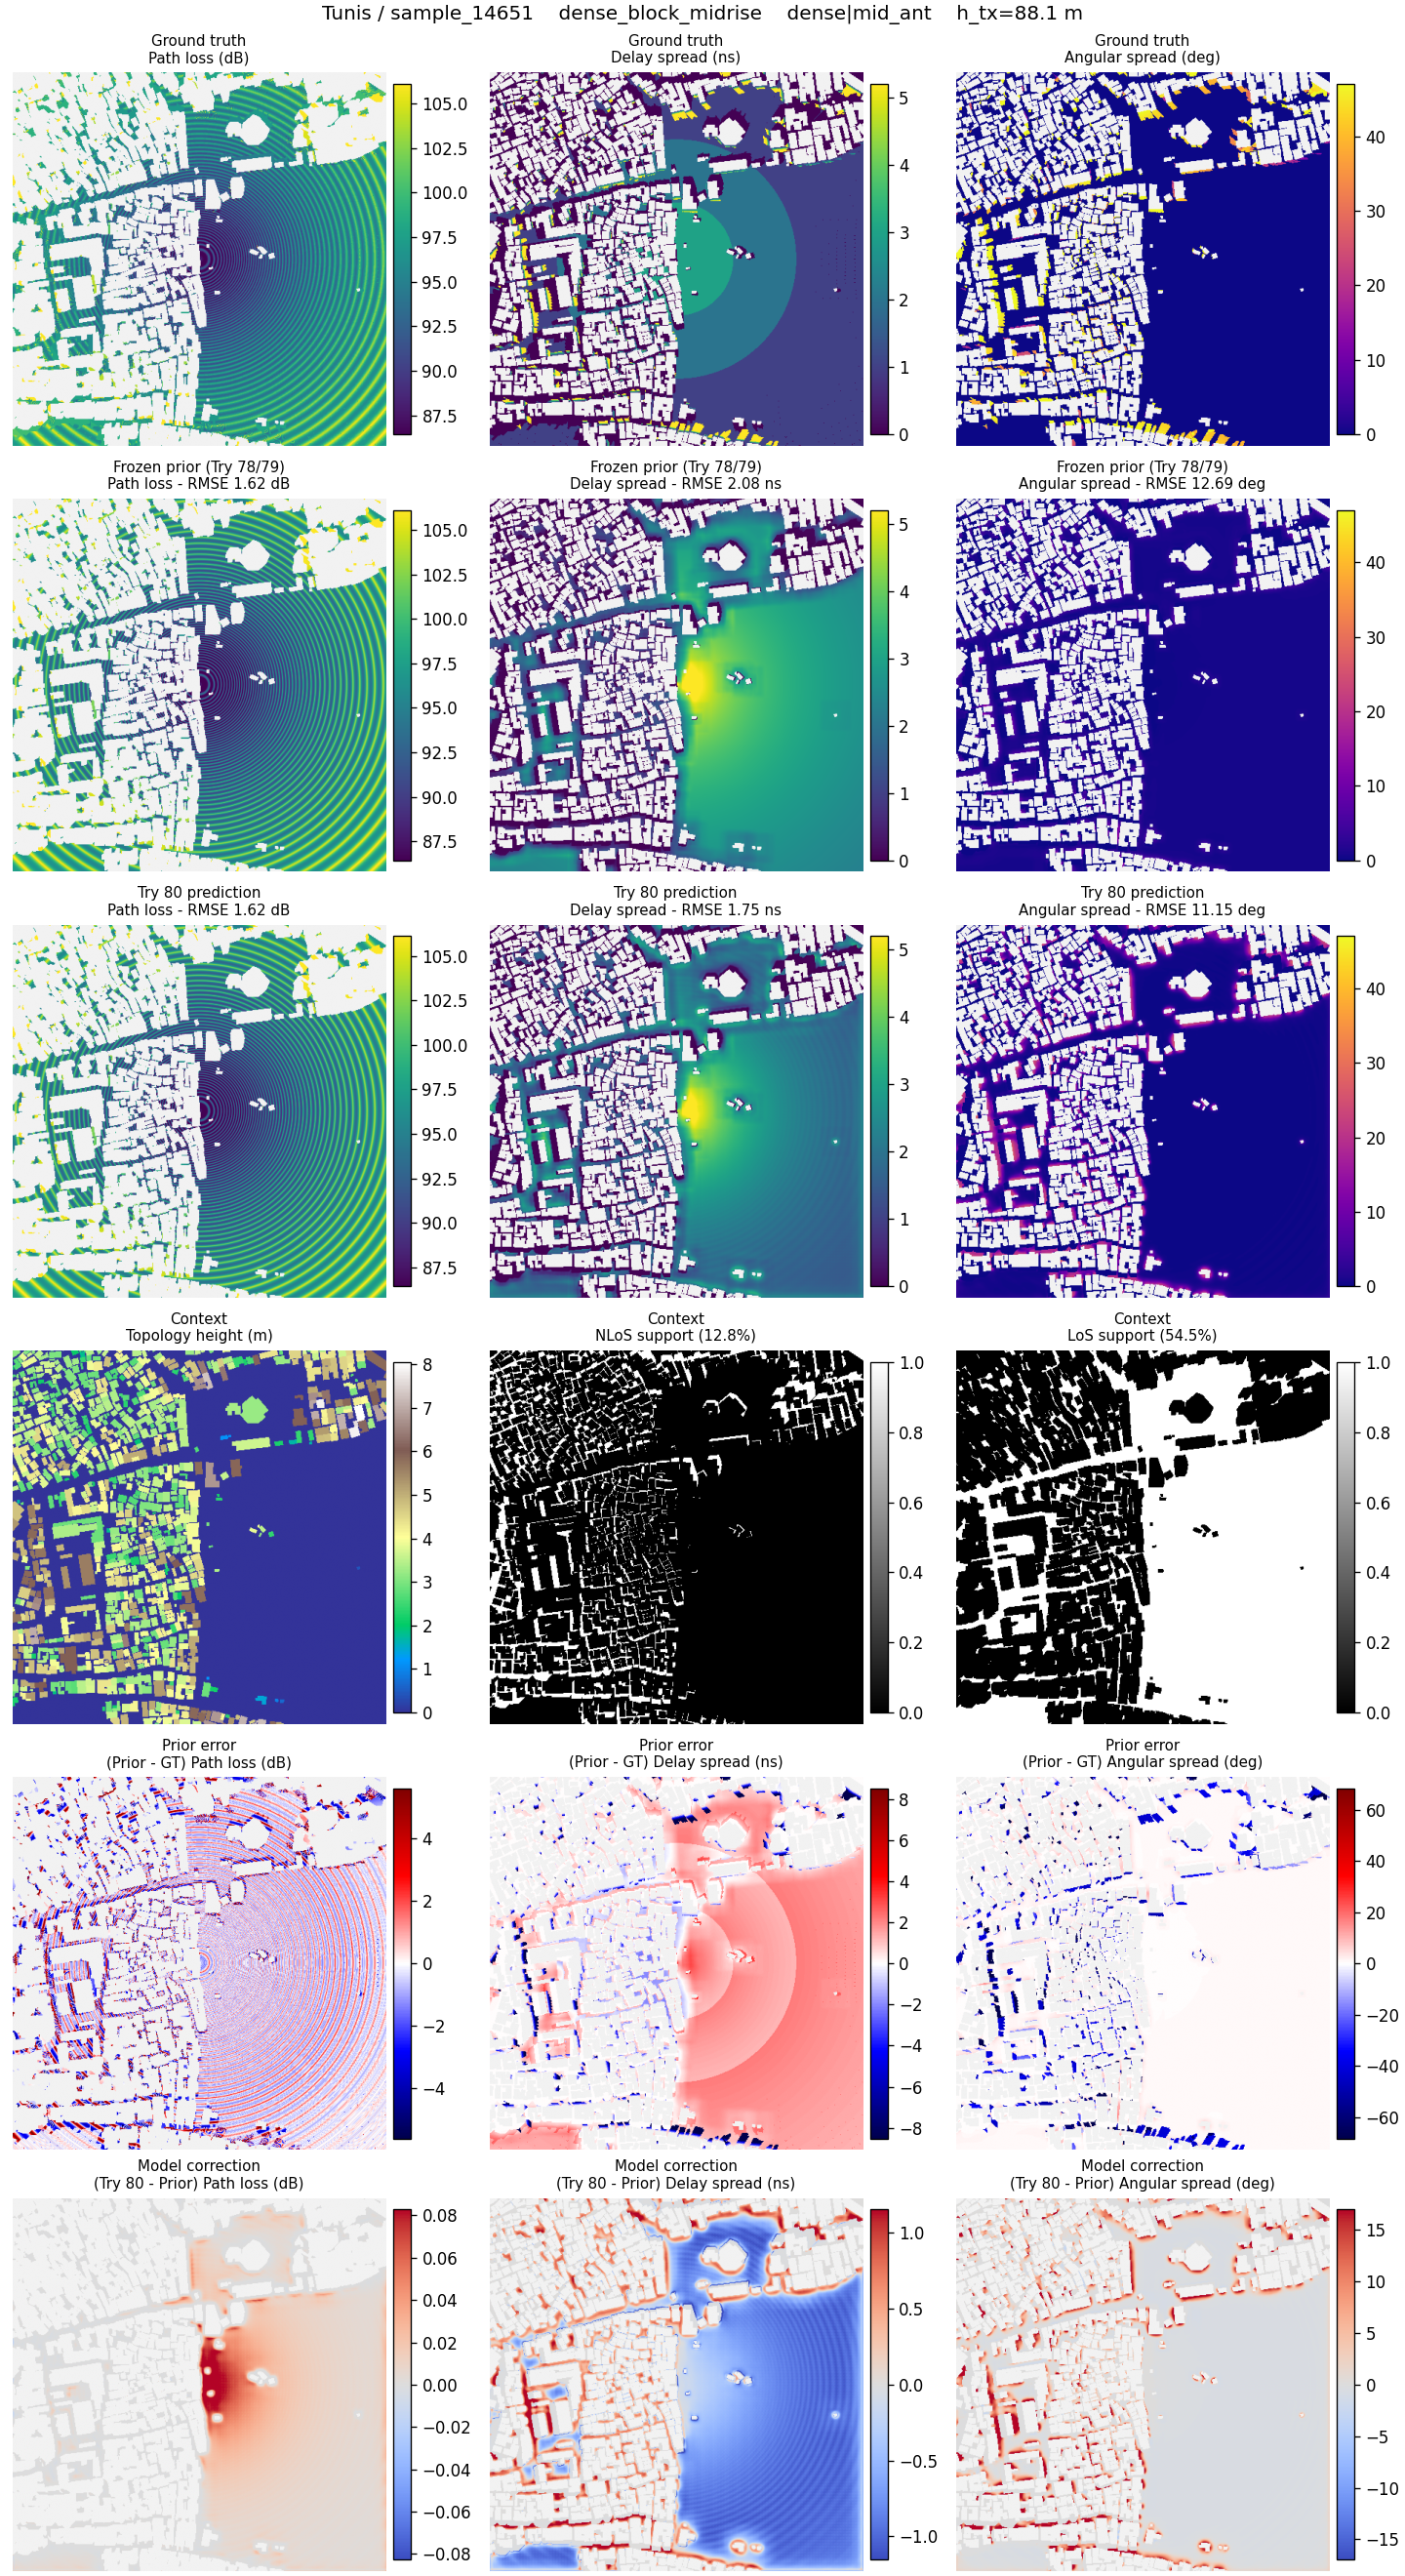
\includegraphics[width=0.92\textwidth,height=0.62\textheight,keepaspectratio]{img/thesis_figures/try80_appendix_panels/try80_panel_dense_mid_ant_Tunis_sample_14651_6x3.png}
\caption{Representative final-model inspection panel for a dense, mid-antenna
validation sample in Tunis. Columns are path loss, delay spread, and angular
spread. Rows show ground truth, frozen prior, final prediction,
context/support, prior error, and model correction.}
\label{fig:panel}
\end{figure*}

\subsection{Runtime}

The final generator was compared against the supplied MATLAB ray-tracing path
on Barcelona layouts at full \(513\times513\) resolution on the same laptop:
an AMD Ryzen~5~5600H CPU and an NVIDIA RTX~3050~Ti Laptop GPU. The surrogate includes
LoS/NLoS mask generation, frozen priors, final neural prediction, and default
numeric export after the checkpoint is loaded once. It runs in \SI{0.88}{s} per
sample versus \SI{99.89}{s} for the local ray-tracing path, a \(113.7\times\)
speed-up under this measurement setup. The ray-tracing row uses the CPU path;
the surrogate row uses the laptop GPU with mixed precision.

\begin{table}[t]
\centering
\caption{Runtime comparison for one full-resolution Barcelona CKM sample on
the same Ryzen~5~5600H / RTX~3050~Ti Laptop hardware.}
\label{tab:runtime}
\scriptsize
\begin{tabularx}{\linewidth}{lXr}
\toprule
Method & Timed path & Time \\
\midrule
MATLAB RT & Pixel receivers outside buildings; PL/DS/AS parsed from paths; CPU path &
\SI{99.89}{s} \\
Final generator & Masks, priors, PL/DS/AS prediction, numeric export; CUDA mixed precision &
\SI{0.88}{s} \\
\bottomrule
\end{tabularx}
\end{table}

\section{Discussion}

The paper version reveals what the full thesis should preserve. The core
argument is not the 80-attempt chronology. It is the chain: strict evaluation
contract, distribution diagnosis, calibrated priors, bounded residual
correction, and held-out-city evidence. Most development history is valuable
only when it supports one of those links.

Several limitations remain. First, the labels come from ray tracing rather than
field measurements, so the result is simulator agreement, not over-the-air
validation. Second, target quantization limits how much sub-unit error
structure can be learned. This is not a limitation of the output layer: the
model outputs continuous PL/DS/AS values. It is a limitation of the stored
labels. For path loss, a \SI{0.9298}{dB} final MAE against labels quantized at
about \SI{1}{dB} is already close to the label step, even though the RMSE still
reveals harder tails. Third, the final model is selected under one
city-holdout split and one final training seed. Fourth, the dataset fixes
frequency, antenna pattern, and simulator assumptions; deployment would require
conditioning or calibration across those variables.

\section{Conclusion}

A dense UAV CKM predictor should not be designed as a generic image generator.
In this setting, the best final result came from a hybrid prior-anchored
formulation: frozen calibrated priors model stable radial, visibility, and
spread-statistical structure; a shared neural model learns bounded residuals
for the remaining local errors. The final model improves the frozen priors on
unseen cities for path loss, delay spread, and angular spread, and produces a
fast full-resolution generator. As a compression of the thesis, this paper
suggests that the full document can be shortened aggressively by keeping the
final design chain and moving most chronological attempt detail to appendices
or repository documentation.

\bibliographystyle{IEEEtran}
\bibliography{../reduced/TFG/TFG}

\end{document}
